\problem{Kinfolk}



The English language abounds with terms for describing family
(genetic) relationships.

The basic relationships are:

\begin{itemize}
\item ``Parent'' and ``child'' are well understood.

\item Children of the same parent are ``siblings''.

\item The child of your sibling is your niece (if she is female) or
  nephew (if he is male). You would be their aunt (if you are female)
  or uncle (if you are male).

\item Two people who share a common grandparent but not a common
  parent are ``1st cousins''.  If they share a common
  great-grandparent but not a common grandparent, they are ``2nd
  cousins''. This can be extended to ``3rd cousins'', ``4th cousins'',
  and so on.
\end{itemize}

These relationships are extended to later generations as follows:

\begin{itemize}

\item The ``child'', ``niece'', and ``nephew'' relationships can be extended
  to later generations by pre-pending ``grand'', ``great-grand'', or
  ``great-great-grand''.  Thus the child of one's child is a
  grandchild. The male child of your niece or nephew is your
  grandnephew. You grandnephew's female child would be your
  great-grandniece, and so on. (In theory, we could extend this to any
  number of additional ``great-'' prefixes, but we will stop with
  ``great-great-grand'' in this problem.)

\item The ``parent'', ``aunt'', and ``uncle'' relationships are extended
  symmetrically by the same prefix. Thus you would be the grandparent
  of your grandchild, the great-granduncle or great-grandaunt of your
  great-grandnieces and great-grandnephews, etc.

\item The ``cousin'' relationship is extended to your cousin's descendants
  by degrees of removal. The children of your 1st cousin are your
  first cousins once removed (and, symmetrically, you are their 1st
  cousin once removed).  The grand-children of your 3rd cousin are
  your 3rd cousins twice removed.The great-grandchildren of your 2nd
  cousin are your 2nd cousins thrice removed. All of the cousin-based
  relationships are symmetric, so if someone is your
  \textit{K}$^{\mbox{th}}$ cousin \textit{something} removed, you are
  theirs as well.
\end{itemize}

Write a program to determine the relationship of one person to another.

\subsection*{Input}

Input will consist of one or more datasets. Each dataset consists of a
single line containing two non-equal integers in the range
$0\ldots \num{32767}$ and a character. A negative number for the first
integer indicates end of input.

The integers identify persons A and B. The character will be either
`M' or `F', designating the gender of person B as male or female.

\begin{wrapfigure}{r}{0.6\linewidth}
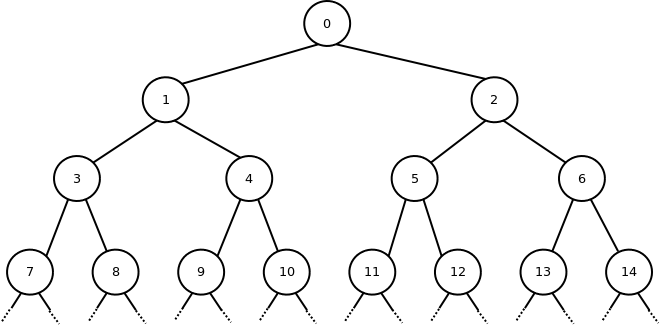
\includegraphics[width=\linewidth]{Kinfolk/fullTree.png}
\end{wrapfigure}

The integers identify the positions of person A and person B in a
family tree envisioned as follows: consider a full binary tree in
which the root is numbered 0, its children are numbered 1 and 2, and
numbering proceeds in that manner, level by level, left to right. This
numbering scheme is shown in the diagram to the right. A parent-child
relationship in this tree represents a parent-child relationship in
the family.


\subsection*{Output}

For each dataset, print a single line indicating the relationship of B
to A.  This relationship must be constructed from the phrases ``child'',
``parent'', ``niece'', ``nephew'', ``aunt'', ``uncle'', ``cousin'', ``grand'',
``great-'', ``1st'', ``2nd'', ``3rd'', ``once removed'', ``twice removed'', and
``thrice removed''.

\begin{itemize}
\item No more than two ``great-'' prefixes may be applied.

\item If  ``1st'', ``2nd'', or ``3rd'' is used, it should be separated from
  the following part of the line by a single blank.

\item If ``once removed'', ``twice removed'', or ``thrice removed'' is used,
  it must be separated from the preceding part of the line by a single
  blank.
\end{itemize}

If it is not possible to describe the relationship of B to A under the
above limitations, then print ``kin''.

\subsection*{Example}

Given the input:

\verbfile{Kinfolk/test0.in}


the output should be:

\verbfile{Kinfolk/test0.expected}



